\clearpage
\section{Results}
We present the results of our empirical analysis for the sample of experts (the WES sample) and the sample of non-experts (the prolific sample).  We estimate the following model by binary logit. 
\begin{equation*}
    Y_{ijc}= \alpha_{j}+ \beta *D_{c} + \gamma*X_{i}
\end{equation*}
Where $Y_{ijc}$ denotes the response of individual $i$ from country $c$ to question $j$. Our answer possibilities either allow individuals to state their level of agreement with a statement or to which party a statement applied. To facilitate interpretation  $Y_{ijc}$ takes a value of one if a participant stated either strongly or slightly agree or if a participant stated the lender countries as the responsible party. We will control for individual characteristics $X_{i}$ such as age, level of education, gender and employment status (affiliation for the expert sample). The dummy variable $D_{c}$ indicates whether the respondents report to have the nationality of one of the lender countries. Consequently, the coefficient $\beta$ measures the impact of lender country nationality on the response $Y_{ijc}$. How can the beta coefficient be interpreted in light of the hypothesis that countries show a nation-serving bias in their assessment of the European debt crisis?  The coefficient $\beta$ shows how much the answers of participants from lender countries deviate from the answers of participants from borrower countries. Since we estimate our model by logit $\beta$ needs to be interpreted as the percentage point difference  in the probability to agree with a statement or state lender countries between borrower and lender countries. If the $\beta$ coefficient is statistically significant and of the predicted sign, we can reject the null hypothesis that there is no nation-serving bias \footnote{Depending on the role as borrower or lender country} in the recollection of the European debt crisis. 
\\ \\
\textbf{Baseline Results} 
Our baseline results corroborate the findings of our descriptive analysis. The divergence between participants from lender and borrower countries on the intentions of the lender countries behind the rescue program are large and statistically significant. As suggested by our descriptive analysis there is little disagreement that the lender countries wanted to avoid a crisis at home.  \\ 
 \begin{figure}[H]
\begin{center}
     \caption{Intentions of the lender countries}
    
     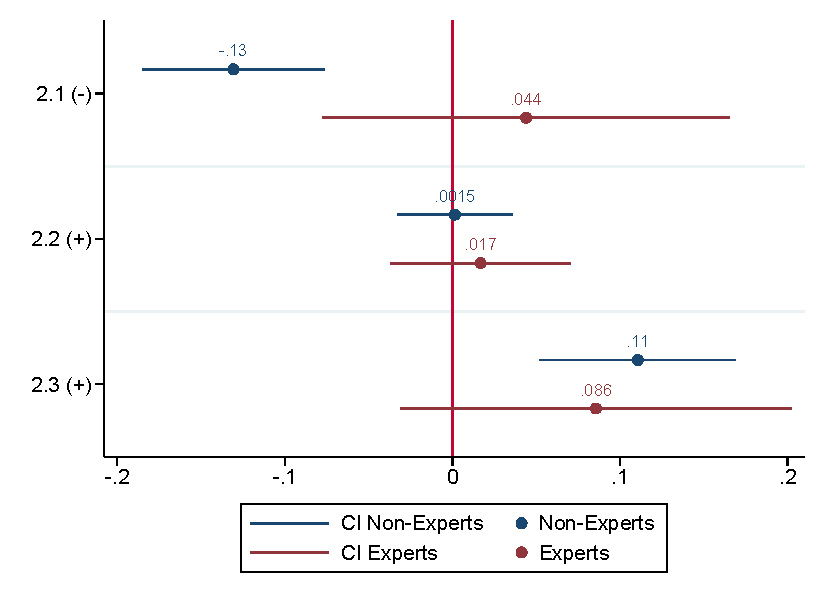
\includegraphics[scale=0.8]{Question2_base.pdf}
     \label{fig:my_label}
      \end{center}
      \tiny
     \tablenotes{The exact wording of the questions were the following.  Question 2.1: The lender countries wanted to help the borrowing countries Question 2.2: The lender countries wanted to help themselves avoid a crisis at home Question 2.3: The lender countries wanted to impose institutional change upon the borrower countries  }
\end{figure}
We proceed to evaluate who initiated and who benefited from the credit relationship. 
In the non-expert sample citizens are 13.2 percentage points more likely to state that the lender countries were the driving force behind signing the memorandum. Further, they are 28 percentage points more likely to state that the lender countries were the main beneficiaries of the program and 20.3 percentage points more likely to state that lender countries benefited from the loans to Greece. All effects are statistically significant at the one percent level. We do not find statistically significant effects in the expert sample. \\
\begin{figure}[h!] 
\begin{center}
     \caption{Who initiated and benefited from the rescue program}
     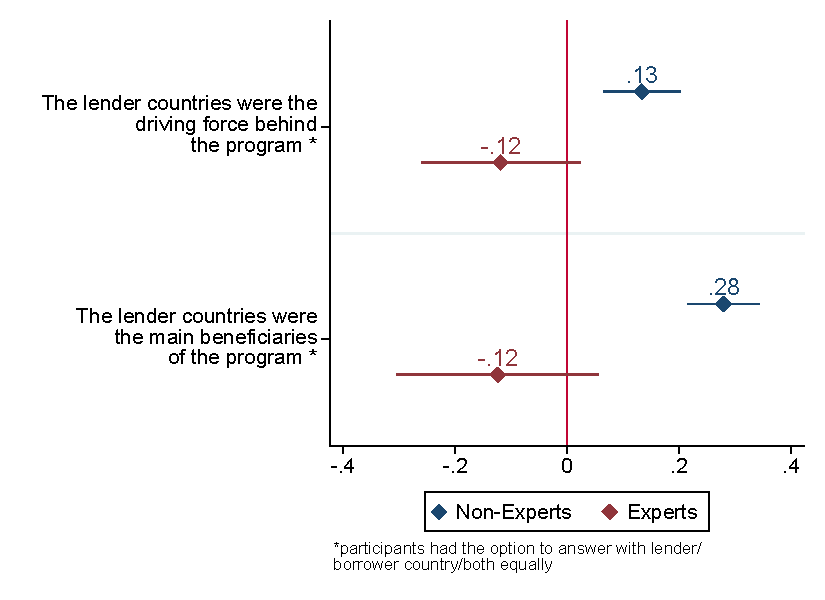
\includegraphics[scale=0.8]{Question3_4_base.pdf}
     \label{fig:my_label}
     \end{center}
     \tiny
     \tablenotes{The sign in parantheses denotes the predicted differential effect.Question 3: Who was the driving force behind signing the memorandum; Question 4: Who was the main beneficiary of the program; Question 7: Who primarily benefited from the loans to Greece}
\end{figure}
We examine how the rescue program influenced the emotions of citizens. Participants from program countries in the non-expert sample are 9.2 and 9.3 percentage points more likely to agree that the rescue experience made them feel guilty and inferior. Further, the probability to agree to "The rescue experience made many citizens in the borrower countries feel exploited" increases by 17 percentage points among citizens from program countries. All effects are statistically significant at the 1 percent level.  \\
As suggested by our descriptive analysis causal inference corroborates that borrower countries do not have a blind spot about the emotions evoked by lender countries.  \\


 \begin{figure} [h!]
    \begin{center}
    \caption{Sentiments of the borrower countries}
    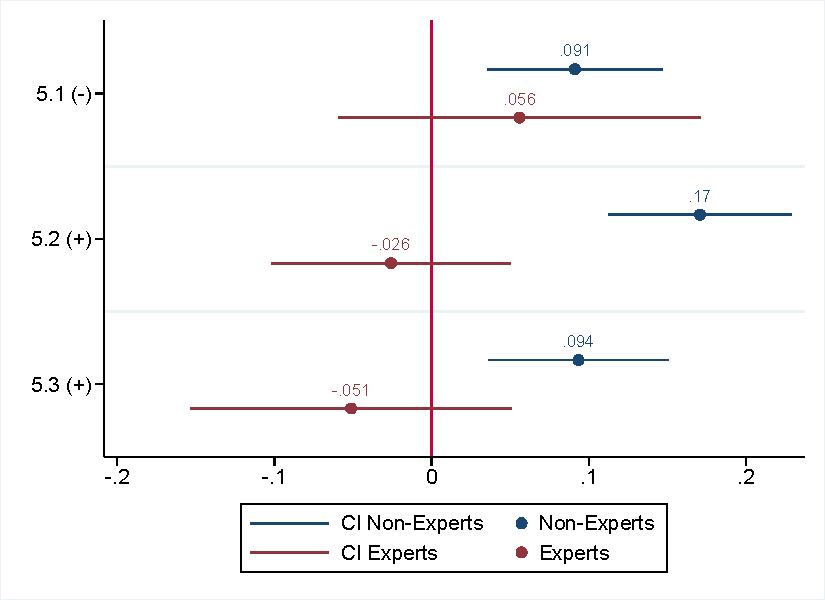
\includegraphics[scale=0.8]{Question5_1_base.pdf}
    \label{fig:my_label}
    \end{center}
    \tiny
    \tablenotes{The exact wording of the questions are the following. Question 5.1: The rescue experience made many citizens in the borrower countries feel guilty; Question 5.2: The rescue experience made many citizens in the borrower countries feel exploited; Question 5.3: The rescue experience made many citizens in the borrower countries feel inferior. }
\end{figure}
\begin{figure}[h!]
\begin{center}
\caption{Sentiments among lender country citizens}

    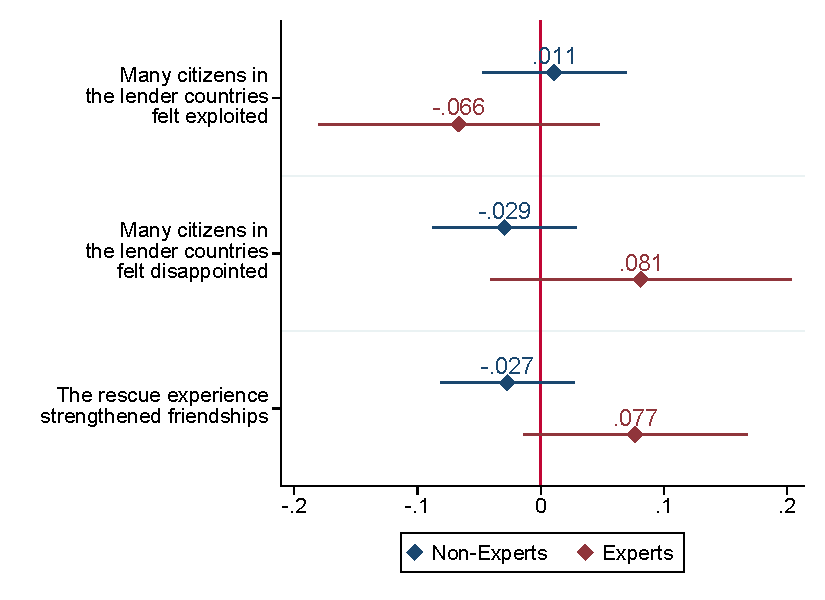
\includegraphics[scale=0.8]{Question5_2_base.pdf}
    \label{fig:my_label}
    \end{center}
    \tiny
    \tablenotes{The sign in parantheses denoted the predicted differential effect. Question 5.4: The rescue experience made many citizens in the lender countries feel exploited; Question 5.5 The rescue experience made many citizens in the lender countries feel disappointed Question 5.6: The rescue experience strengthened friendships between citizens Question 7: Greece will fully pay back it's debt}
\end{figure}
 
%  \begin{figure}
%\caption{Assessment of the emotions the program evoked among different parties}
%\centering
%\begin{minipage}{.5\textwidth}
% 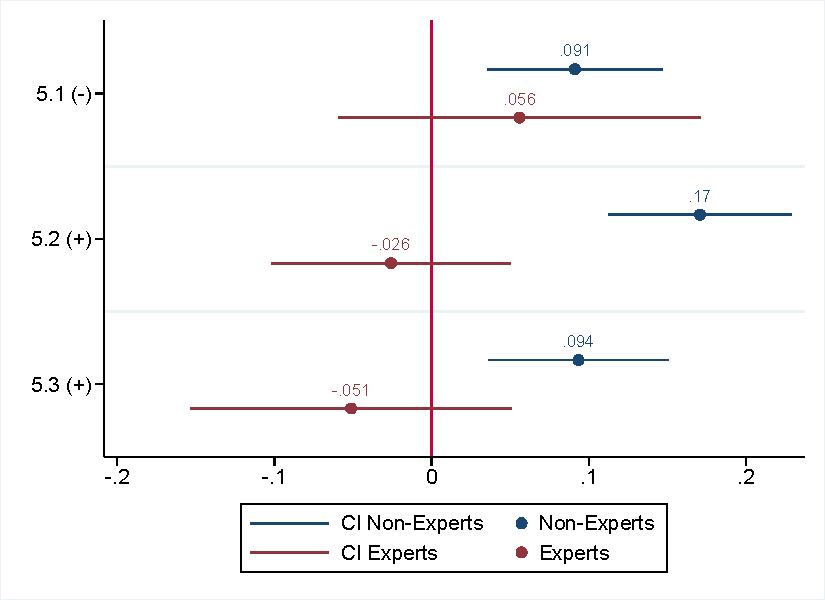
\includegraphics[scale=0.5]{Question5_1_base.pdf}
 %\end{minipage}%
 %\hfill
%\begin{minipage}{.5\textwidth}
%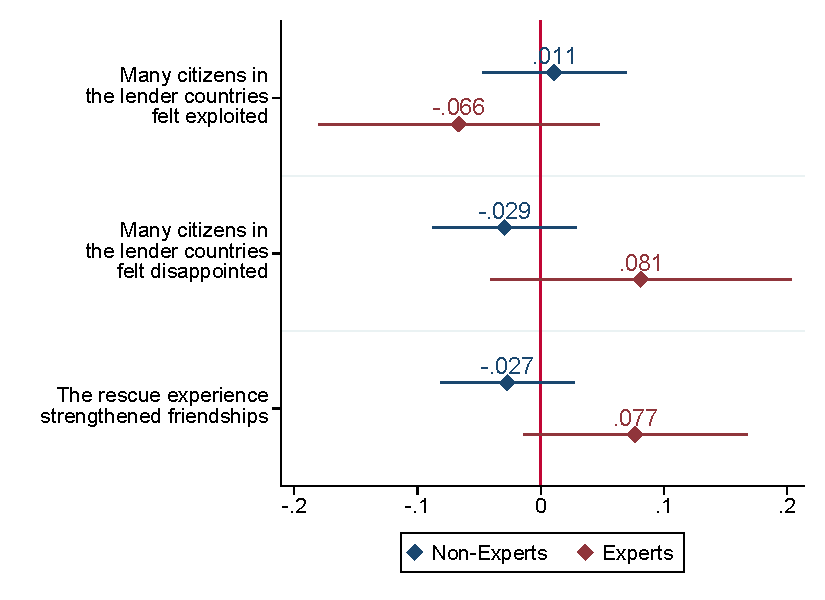
\includegraphics[scale=0.5]{Question5_2_base.pdf}
%\end{minipage}
%\end{figure}
 \clearpage
 The interpretation of the outcomes of our questions regarding the situation in Greece are not straightforward. We find that lender countries are 20 percentage points more likely to state that the lender countries were the primary beneficiaries from the loans to Greece. It is noteworthy, that the difference between lender countries and borrower countries is slightly smaller when they are specifically asked about Greece, than when the question is asked more generically. Participants from borrower and lender countries diverge if Greece will be able to fully repay its debt. For the first time, the observed difference is statistically significant for both samples. 
 \\
\begin{figure}[h!] 
\begin{center}
     \caption{Situation in Greece}
     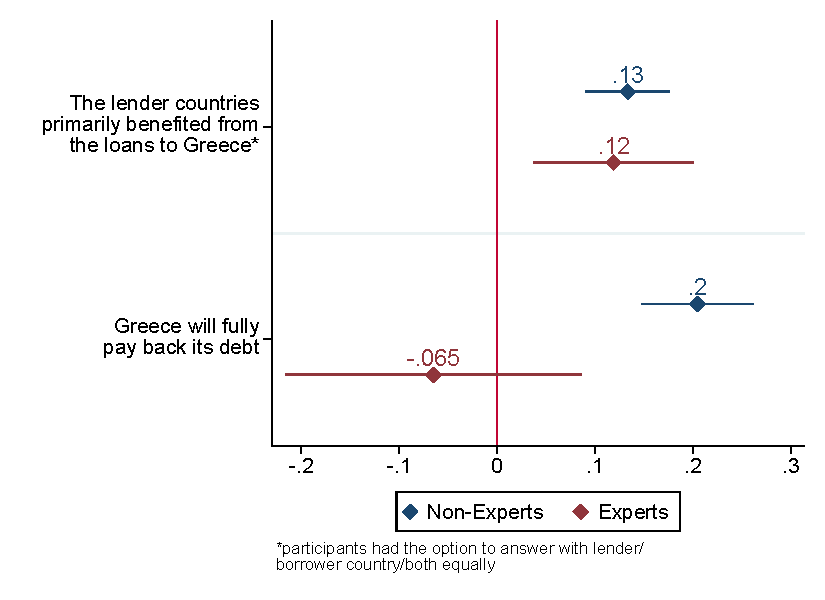
\includegraphics[scale=0.8]{Question6_7_base.pdf}
     \label{fig:my_label}
     \end{center}
     \tiny
     \tablenotes{The exact wording of the question was the following.   Question 6: Who primarily benefited from the loans to Greece; Question 7: Greece will fully pay back it's debt}
\end{figure}
\clearpage
\section{Heterogeneity Analysis}
 
The results of our multivariate analysis illustrate that the non experts show a strong nation-serving bias in their recollection of the European debt crisis along various dimensions. This nation-serving bias is largely absent among the sample of experts. The divergence between  the assessments of experts and non-experts has been investigated by \cite{roth}. The authors compare survey results from the WES and a representative sample and find that experts differ from non-experts in their beliefs about the impacts of macroeconomic shocks. However, in contrast to \cite{roth} the purpose of our study is not to investigate how well average citizens understand economics but rather how a very intrusive economic event and its consequences are perceived and remembered.
In the following we investigate several explanations for why we can only observe the nation-serving bias among our sample of non-experts. 
We start by evaluating which socioeconomic characteristics inherent to experts might explain why we observe a smaller nation-serving bias among them. For this purpose we conduct sample splits to check whether certain subparts of the population show a stronger nation-serving bias than others.
\\

 According to \cite{baumeister} events experienced at a younger age might have a more defining impact. Since the European debt crisis was accompanied for example by a high level of youth unemployment it might seem plausible that the divergences in memory might be more pronounced among the younger generation. Thus, we estimate the effect of belonging to a program country among participants older than 35 among the sample of non-experts.  The effect of the program variable on the likelihood to agree that the lender countries wanted to impose institutional change or that the rescue experience made citizens in the borrower countries feel guilty is smaller and the significance level decreases to 5 percent. For the remaining questions the overall magnitude and significance level of the program effect stays the same. 
\\
The level of education of participants may well influence the estimates. Participants with a higher level of education might have different political attitudes or consume and access different types of media. Hence, we split the non-expert sample and estimate our model only for participants reporting to have completed tertiary education. We do not find any change in the magnitude and significance level of effects for this subsample. 
\\
One dimension along which experts and non-experts differ is their degree of mobility. Experts working in think tanks or research institutes might live or have studied abroad for some time. Due to this circumstance experts might identify less with their nation than non-experts and consequently will not have a strong nation-serving bias. Previous studies such as the one by \cite{bechtel} have shown that having a cosmopolitan attitude was a strong predictor of citizens' attitudes towards the rescue program. Citizens with a more cosmopolitan attitude were more willing to accept international redistribution in the form of financial loans than people with a less cosmopolitan attitude. Unfortunately, we did not include a measure of sharing cosmopolitan attitudes in our survey. However, we can identify if participants reported to be living in a different country than their country of birth which presents us with a proxy. Overall 541 participants reported living in a different country than their country of birth. 437 of these participants are from borrower countries and 104 are from lender countries. The fraction of participants living in a different country than their country of birth is more or less equally distributed among borrower countries. For lender countries the highest fraction of mobile participants come from Eastern European countries. Estimating our model for this subsample changes the results quite a bit. Divergence between citizens from borrower and lender countries remains in the assessment if lender countries wanted to help borrowing countries and if the rescue experience made the citizens in the borrower countries feel exploited. For the other questions the difference in answers between program- and non-program countries becomes smaller and even vanishes completely for some questions. Hence, it appears that, consistent with previous studies, participants who are more mobile and more cosmopolitan display a lower nation-serving bias.  \\

We also control whether participants beliefs about the status of their country increase the magnitude of results. One might expect that citizens who are accurately informed about their country's status as a lender or borrower country might display a stronger nation-serving bias. Restricting the sample to participants who correctly stated whether their country had borrower or lender status does not yield substantially different results as the baseline estimates. We also redefine the dummy variable according to people's beliefs about the status of their country. We then investigate whether we find significant divergence between citizens who believe to live in a lender country and citizens who believe to live in a borrower country. Overall we find a smaller effect after this redefinition than in our original baseline estimates. The only significant divergence between participants who believed to be living in lender countries and participants who believed to be living in borrower countries can be found in the assessment of the emotions the rescue program evoked among the lender countries. These findings are interesting with regards to identifying the origin of a nation-serving bias. It appears that identifying as borrower or lender does not drive the results but rather that the recollection of the European debt crisis is influenced by subconscious factors. 
\\
Overall it appears that the absence of a nation-serving bias among the expert sample does not seem to be driven by differences in socioeconomic characteristics such as age or education but rather other factors. One potential factor which might explain the divergence in opinions is the fact that experts might be exposed to a more international environment. This is corroborated by our finding that non-experts who were born in a different country than their current country of residence show a lower degree of nation-serving bias than the full sample. These findings are very much in line with other studies such as the one by \cite{bechtel} who show that support for international redistribution increases with more cosmopolitan attitudes. These people might not define themselves as strongly via their nationality than people with less cosmopolitan attitudes and thus have a different view on international policies. 

